% ****** Start of file aipsamp.tex ******
%
%   This file is part of the AIP files in the AIP distribution for REVTeX 4.
%   Version 4.1 of REVTeX, October 2009
%
%   Copyright (c) 2009 American Institute of Physics.
%
%   See the AIP README file for restrictions and more information.
%
% TeX'ing this file requires that you have AMS-LaTeX 2.0 installed
% as well as the rest of the prerequisites for REVTeX 4.1
%
% It also requires running BibTeX. The commands are as follows:
%
%  1)  latex  aipsamp
%  2)  bibtex aipsamp
%  3)  latex  aipsamp
%  4)  latex  aipsamp
%
% Use this file as a source of example code for your aip document.
% Use the file aiptemplate.tex as a template for your document.
\documentclass[%
aip,
jmp,%
amsmath,amssymb,
%preprint,%
reprint,%
%author-year,%
%author-numerical,%
]{revtex4-1}

%\usepackage[superscriptaddress]{revtex4-1-mod}
\usepackage[brazil]{babel}
\usepackage[utf8]{inputenc}
\usepackage{graphicx}% Include figure files
\usepackage{dcolumn}% Align table columns on decimal point
\usepackage{bm}% bold math
\usepackage{comment}
\usepackage{tikz}
%\usepackag[brazil]{babel}
\usepackage{graphicx}
\usepackage{epstopdf}
%\def\Dated@name{Data: }
%\usepackage[mathlines]{lineno}% Enable numbering of text and display math
%\linenumbers\relax % Commence numbering lines
\newcommand{\dd}{\,\mathrm{d}}
\renewcommand{\arraystretch}{1.2}
%\documentclass[a4paper]{article}
\usepackage{xcolor}
% Definindo novas cores
\definecolor{verde}{rgb}{0,0.5,0}
% Configurando layout para mostrar codigos C++
\usepackage{listings}
\lstset{
	language=C++,
	basicstyle=\ttfamily\small, 
	keywordstyle=\color{blue}, 
	stringstyle=\color{verde}, 
	commentstyle=\color{red}, 
	extendedchars=true, 
	showspaces=false, 
	showstringspaces=false, 
	numbers=left,
	numberstyle=\tiny,
	breaklines=true, 
	backgroundcolor=\color{green!10},
	breakautoindent=true, 
	captionpos=b,
	xleftmargin=0pt,
}

%\usepackage[mathlines]{lineno}% Enable numbering of text and display math
%\linenumbers\relax % Commence numbering lines
\begin{document}
	
	\preprint{AIP/123-QED}
	
	\title[Códigos de Bloco]{Códigos de Bloco}
	\thanks{Auxílio matemático: Introdução à terceira atividade laboratorial de ELE-32. Dispon\'ivel em \url{https://goo.gl/Xe8c5i}.}% Force line breaks with \\
	%\thanks{Folha de aux\'ilio: Manual de Instru\c{c}\~oes e Guia de Experimentos AZEHEB. Dispon\'ivel em \url{http://goo.gl/GWAc8w}.}
	\author{Dennys L. A. Rocha}
	%\altaffiliation[Aluno de gradua\c{c}\~ao do ]{Instituto Tecnol\'ogico de Aeron\'autica}%Lines break automatically or can be forced with \\
	\thanks{Endereço eletrônico: dennysrocha.1994@gmail.com}
	
	\author{Gabriel Adriano de Melo}%
	%\email{Second.Author@institution.edu.}
	%\affiliation{Alunos de gradua\c{c}\~ao do Instituto Tecnol\'ogico de Aeron\'autica}
	%Authors' institution and/or address%\\This line break forced with \textbackslash\textbackslash
	\thanks{Endereço eletrônico: gaadrime.melo@gmail.com}
	
	
	%\homepage{http://www.Second.institution.edu/~Charlie.Author.}
	\affiliation{Alunos de gradua\c{c}\~ao do Instituto Tecnol\'ogico de Aeron\'autica}
	%Second institution and/or address%\\This line break forced% with \\
	
	
	\date{17 de novembro de 2017}% It is always \today, today,
	%  but any date may be explicitly specified
	
	\begin{abstract}
		
		Neste trabalho estudou-se a decodificação (correção de erros) de sinais que passam por canais ruidosos. Para isso, empregou-se o método de \textit{Hamming (7,4,3)} como solicitado no pré-relatório e também um código de livre escolha, o \textit{Golay (24,12,8)}. Os algoritmos criados foram feitos nas linguagens \textit{Java} e \textit{MATLAB}. Eles operam de modo a gerar textos binários aleatórios e trabalhar sobre eles adicionando ruídos e corrigindo seus erros.\\[5pt]
		\noindent
		Palavras-chave: Hamming, Golay, erro.\\[5pt]
		\noindent
		
		
		In this work we studied the decoding (error correction) of signals passing through noisy channels. For that, the Hamming method (7,4,3) was used as requested in the pre-lab and also a free choice code, the Golay (24,12,8). The algorithms were created in Java and MATLAB languages. They operate in order to generate random binary texts and work on them by adding noise and correcting their errors.\\[5pt]
		\noindent
		Keywords: Hamming, Golay, error.\\[5pt]
	\end{abstract}
	
	\maketitle
	
	\section{\label{sec:level1}introdu\c{c}\~ao}
	
	No estudo das comunicações digitais, nôs deparamos com métodos de correção para erros gerados na transmissão de uma mensagem. Neste relatório serão estudados os métodos de Hamming (7,4,3) e Golay (24,12,8) (por simplicidade serão chamados respectivamente de Hamming e Golay apenas).
	
	O método de Hamming utiliza código de 4 bits (chamado de palavra) e sua palavra-código possui 7 bits. Ele é capaz de corrigir um erro e detectar até dois. Seu modo de funcionamento se baseia em, dados os 4 bits de código, adicionar mais três bits (chamados bits de paridade) para correção de erros.
	
	De forma semelhante ao método de Hamming, o método de Golay também trabalha com bits de redundância, mas este opera com códigos de 12 bits e palavras-código de 24 bits. Ele é capaz de corrigir até três erros e detectar sete.
	
	Os números que acompanham os nomes dos métodos são, respectivamente, o tamanho da palavra-código (n), o tamanho do código (k) e a distância mínima entre duas palavras-código (r). Define-se como taxa a razão entre o tamanho do código e o tamanho da palavra-código (Equação \ref{eq:taxa}):
	
	\begin{equation}
		R = \frac{k}{n} \label{eq:taxa}
	\end{equation}
	
	Ambos os códigos atuam de modo a corrigir erros gerados pelo canal onde a mensagem passa, então é razoável definir um parâmetro que meça o quanto de informação errônea foi transmitida, comparando-se a mensagem enviada da mensagem recebida. Esse parâmetro é chamado de \textit{Bit Error Rate} (BER) e é definido pela Equação \ref{eq:ber}:
	
	\begin{equation}
		BER = \frac{N_{erros}}{N} \label{eq:ber}
	\end{equation}
	
	onde $N_{erros}$ é a quantidade total de bits trocados e $N$ a quantidade total de bits transmitidos.
	
	
	
	\section{Descrição dos algoritmos}
	
	Nesta atividade, foi utilizado um canal binário simétrico (BSC), onde a probabilidade de troca de bit independe do valor do bit. Os códigos transmitidos pela fonte são tratados ao passar por esse canal. Cada um dos códigos deve estimar, a partir de seu método de correção, quais bits foram trocados e corrigi-los.
	
	\subsection{Método de Hamming}
	Para o codificador de Hamming, devemos gerar os bits de paridade conforme ilusta a Figura \ref{fig:hammingdiagrama}.
	
	\begin{figure}[h]
		\centering
		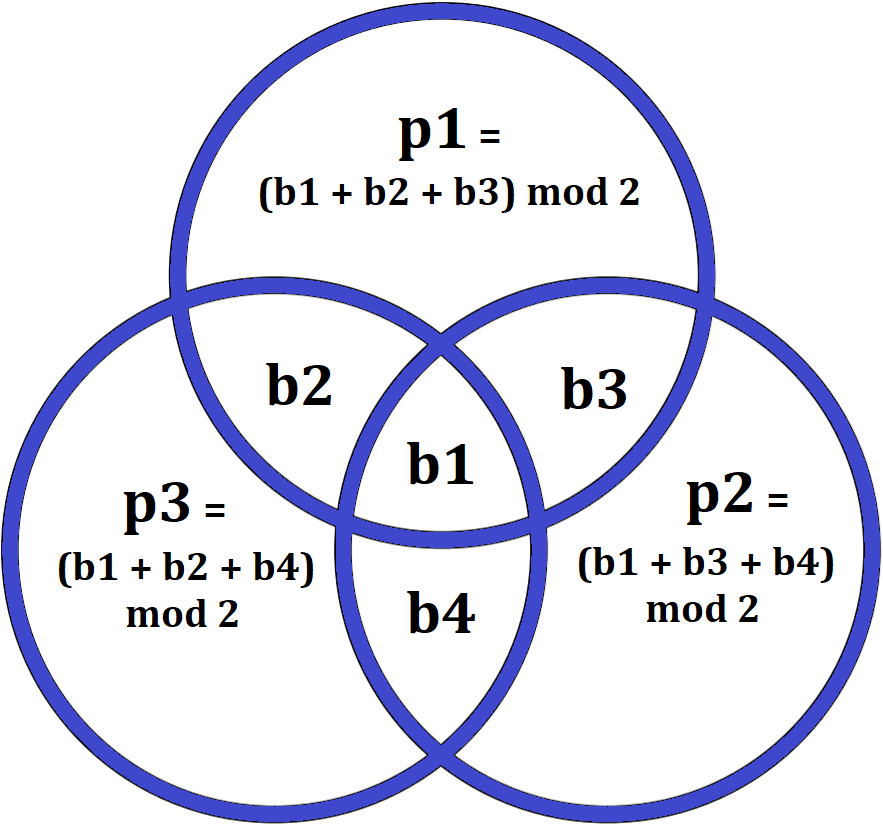
\includegraphics[width=0.48\textwidth]{images/hamming}
		\caption{Diagrama ilustrativo para a construção dos bits de paridade e assim a palavra código.}
		\label{fig:hammingdiagrama}
	\end{figure}
	
	De modo a gerar os bits de paridade, constrói-se uma matriz de paridade $G$ de tal forma que todas as colunas de comprimento 4 sejam linearmente independentes. Essa matriz, ao ser multiplicada pelo vetor código $v_{1\times4}$, deve retornar um vetor $w_{1\times7}$ chamado de palavra-código, que tem a informação nos quatro primeiros bits e as paridades nos três últimos, isto é:	
	\begin{equation}
		w = v\cdot G = b_{1}b_{2}b_{3}b_{4}p_{1}p_{2}p_{3}
	\end{equation}
	
	A mensagem w é então enviada ao decodificador que, com uma matriz	
	\begin{equation}
	H^{T} = \left[\begin{array}{ccc}
	1 & 1 & 1 \\
	1 & 0 & 1 \\
	1 & 1 & 0 \\
	0 & 1 & 1 \\
	1 & 0 & 0 \\
	0 & 1 & 0 \\
	0 & 0 & 1
	\end{array}
	\right]
	\end{equation}
	
	encontra a síndrome	
	\begin{equation}
		s = w\cdot H^{T}
	\end{equation}
	
	que, devido à propriedade $v\cdot H^{T}=0_{1\times3}$, se simplifica a Equação \ref{eq:sindrome}:	
	\begin{equation}
		s = e\cdot H^{T} \label{eq:sindrome}
	\end{equation}
	
	onde $e$ é o erro gerado pelo canal.
	
	A partir da síndrome obtida, decide-se qual é o erro fazendo a suposição de que ele terá peso de Hamming igual a 1.
	
	A mensagem estimada será, portanto, dada pela Equação \ref{eq:hamming}	
	\begin{equation}
		v \equiv w+e\; (mod\, 2) \label{eq:hamming}
	\end{equation}
	
	\subsection{Método de Golay}
	
	Semelhante ao método de Hamming, no método de Golay usa-se uma matriz de paridade
	\begin{equation}
	G = \left[I_{12}\:|\left(\begin{array}{cccc}
	A_1|1&A_2|1&...&A_{12}|1
	\end{array}\right)^{T}\right]
	\end{equation}
	
	cujos $A_{i}$, $i=1,...,11$, são obtidos sucessivamente através do vetor
	
	\begin{equation}
		A_1 = \left[1\begin{array}{ccccccccccc}
		1&1&0&1&1&1&0&0&0&1&0
		\end{array}\right]
	\end{equation}
	
	mudando a posição do primeiro elemento para a última posição e com $A_{12}$ um vetor com apenas a ultima coluna igual a zero:
	
	\begin{equation}
		A = \left[\begin{array}{cccccccccccc}
		1&1&0&1&1&1&0&0&0&1&0&1 \\
		1&0&1&1&1&0&0&0&1&0&1&1 \\
		0&1&1&1&0&0&0&1&0&1&1&1 \\
		1&1&1&0&0&0&1&0&1&1&0&1 \\
		1&1&0&0&0&1&0&1&1&0&1&1 \\
		1&0&0&0&1&0&1&1&0&1&1&1 \\
		0&0&0&1&0&1&1&0&1&1&1&1 \\
		0&0&1&0&1&1&0&1&1&1&0&1 \\
		0&1&0&1&1&0&1&1&1&0&0&1 \\
		1&0&1&1&0&1&1&1&0&0&0&1 \\
		0&1&1&0&1&1&1&0&0&0&1&1 \\
		1&1&1&1&1&1&1&1&1&1&1&1
		\end{array}
		\right]
	\end{equation}
	
	O código $v_{1\times12}$ se transforma então na palavra-código $w_{1\times24}$. Para decodificá-la, utilizamos os seguintes passos:
	
	1. Computamos a primeira síndrome:
	\begin{equation}
		s_{1} \equiv w\cdot G^{T}\;(mod\:2)
	\end{equation}
	onde, nesse caso, $H=G^{T}$.
	
	2. Se o peso de Hamming da primeira síndrome for  menor ou igual a três, então o padrão de erro será
	\begin{equation}
		u = \left[s_{1}\:|\:\begin{array}{cccccccccccc}
	0&0&0&0&0&0&0&0&0&0&0&0
	\end{array}\right].
	\end{equation}
	
	3. Se o peso de Hamming da primeira síndrome for maior ou igual a três mas para algum $i=1,...,12$ o peso de Hamming de $s+A_{i}$ for menor ou igual a dois, então o padrão de erro será
	\begin{equation}
		u_1=\left[s+A_{i}\:|\:e_{i}\right]
	\end{equation}
	onde $e_i$ é a i-ésima linha da matriz $I_{12}$. A mensagem é, portanto:
	\begin{equation}
	v \equiv w+u_1\; (mod\, 2)
	\end{equation}
	
	4. Computamos a segunda síndrome:
	\begin{equation}
		s_2 = s\cdot A
	\end{equation}
	
	5. Se o peso de Hamming da segunda síndrome for menor ou igual a três, então o padrão de erro será
	\begin{equation}
		u_2 = \left[\begin{array}{cccccccccccc}
		0&0&0&0&0&0&0&0&0&0&0&0
		\end{array}\:|\:s_{2}\right].
	\end{equation}
	
	A mensagem é, portanto:
	\begin{equation}
	v \equiv w+u_2\; (mod\, 2)
	\end{equation}
	
	6. Se o peso de Hamming da segunda síndrome for maior ou igual a três mas para algum $i=1,...,12$ o peso de Hamming de $s_{2}+A_{i}$ for menor ou igual a dois, então o padrão de erro será
	\begin{equation}
	u_3=\left[e_{i}\:|\:s_{2}+A_{i}\right]
	\end{equation}
	
	A mensagem é, portanto:
	\begin{equation}
	v \equiv w+u_3\; (mod\, 2)
	\end{equation}
	
	7. Caso contrário, reenviar a mensagem da forma que foi recebida ou então, se possível, pedir retransmissão.
	
	\section{resultados\label{sec:resultados}}
	
	1. Qual foi a maior dificuldade de implementar o decodificador para o código de Hamming?
	Para a implementação do código de Hamming, a matriz Ht foi escrita na forma de $(2^n)-1$ linhas por n colunas, de forma que todas as combinações de vetores independentes possíveis fossem escritas, a menos do vetor nulo. Para facilitar na decodificação, escreveu-se os vetores em ordem decrescente (a partir do vetor todo 1), a exceção dos vetores com peso de Hamming unitário, que foram escritos na forma de uma matriz identidade nas últimas linhas.
	Assim, a maior dificuldade, foi que ao contar a síndrome e relacionar com o erro, fazia-se uma contagem decrescente a partir do vetor todo 1, decrementando-o, e dever-se-ia pular os vetores de Hamming com peso um nessa contagem.
	
	2. Qual foi o método utilizado para encontrar o código maior? Este método é extensível para qualquer tamanho de bloco?
	
	O primeiro método consistia em determinar um conjunto de vetores de tamanho n e distância de Hamming mínima k entre eles. Nesse método, partia-se de um vetor inicial de tamanho n com todos os elementos unitários e decrementava-se, verificando se o resultado tinha distância de Hamming k entre todos os vetores da lista em construção (cujo primeiro elemento era o vetor inicial), e em caso afirmativo, adicionava-o à lista. Com a lista concluída, fazia-se uma outra seleção, construindo-se uma lista de todas as síndromes possíveis, com elementos iniciais de peso de Hamming 1 (erros de apenas um bit), em seguida realizando todas as combinações de até Q elementos da lista anterior. Assim, gerava-se uma relação entre as síndromes e os erros nos bits. 
	Utilizou-se o tipo unsigned long long int para essas operações de vetores de bit, representando um vetor de bit de tamanho até 64. A princípio, utilizando-se uma representação maior que 64 bits, esse método é extensível para qualquer tamanho de bloco n, sendo selecionados vetores com distâncias mínima k, realizando-se Q combinações entre eles. 
	
	3. Qual é a relação medida entre o tamanho do bloco e o desempenho?
	Para o código de Hamming, que corrige apenas um erro, um aumento no tamanho do bloco significava uma melhor taxa de transmissão, porém com uma maior taxa de erro de bits.
	Para o algoritmo de seleção de códigos com distância mínima k, verificou-se mais correções de erros de bits com o aumento de k.
	
	4. Como o seu código se compara com a capacidade do canal? Utilize uma probabilidade de erro de bit de $10^-5$.
	A capacidade do canal binário simétrico pode ser calculada por $1 + p log2 p  + (1 - p) log2 (1 - p)$, o que resulta em 0.99982 bit por uso de canal, para a probabilidade de erro de bit de $10^-5$. A nossa implementação do código de Golay utiliza uma taxa de $50 percento$, corrigindo até 3 erros em um bloco, diminuindo a taxa de erro de bits de $10^-5$ para ?????. Assim, temos uma capacidade de aproximadamente 0.5 bit por uso de canal.
	
	5. Qual é a complexidade de codificação e decodificação do seu sistema?
	Para o primeiro método de seleção por força bruta, encontrados os v elementos de tamanho n e de distância k, a codificação se reduz a uma multiplicação de matrizes, com ordem $O(n*v)$ e a decodificação se resumia a uma outra multiplicação de matrizes de ordem $O(n*v)$ e uma busca de síndrome na tabela, de $O(1)$. A complexidade estava em achar tais elementos (construir a matriz g), de ordem $O(2^n)$ e na construção da tabela de ordem $O(v^Q)$.
	Para a nossa implementação de Golay 24, Dennys????
	
	
	\section{Conclus\~ao}
	
	
	
	
	
\flushleft
\flushleft

\pagebreak
\newpage
\newpage

\cleardoublepage
\phantomsection
\addcontentsline{toc}{chapter}{bibliografia}
\bibliographystyle{ieeetr}
\bibliography{bibliografia}

\end{document}
%
% ****** End of file aipsamp.tex ******
